%************************************************
\section*{Methodology}\label{ch:methodology}
%************************************************

The purpose of this chapter is to first formulate the research questions that we examine in our work
and then propose our method of answering them.

\subsection*{Research Questions}\label{sec:research_questions}

In the commit-feature interaction chapter we dicussed the different meanings of structural and dataflow-based interactions.
With this knowledge, we can answer many interesting research topics. 
These topics include patterns in feature development and usage of commits therin as well as findings about how likely seemingly unrelated commits are to affect features inside a program.

\subsubsection*{\textbf{RQ1: How do commits and features structurally interact with eachother?}}

We intend to research two main properties which already provide a lot of insight into the development process of features and usage of commits therein.
Firstly, we examine the amount of commits features interact with structurally.
This gives us a direct estimate on how many commits were used in the development of a feature.
Our analysis also allows us to measure the scope of feature, which can put the amount of commits used to implement a feature into perspective.
Secondly, we want to examine how many features a commit interacts with structurally, e.g. how many features a commit usually changes. 
This is especially interesting when considering best practices surrounding the usage of commits.
It is preferred to keep commits granular\cite{GitBestPractices2023} meaning they should only fix a single bug or, in our case, change a single feature.
Acquiring data on this issue might show how strictly this policy is enforced in the development of features. 

\subsubsection*{\textbf{RQ2: How do commits interact with features through dataflow?}}

Investigating dataflow can unveil interactions between parts of a program that were previously hidden from programmers.
This can help a programmer understand the extent to which new changes affect other parts of a program.
Deploying the introduced analysis in a direct manner could even aid a programmer when fixing bugs of features.
Bugs occuring in certain features could be traced back to their cause by factoring in recent changes affecting said features through dataflow. \\
Previous research has laid the groundwork for researching dataflow interactions between different parts of a program.
However, it has focused solely on dataflow interactions between commits.
That's why we want to provide first insights on the properties of dataflow-based commit-feature interactions.
Specifically, we investigate how connected commits and features are by analyzing the amount of features a commit usually affects through dataflow.
Knowing what fraction of all commits contributing code to a project are part of dataflow-based interactions can show how often new commits affect the data of a feature. 
Regarding this, it is worth considering that commits constituting code of a feature are very likely to influence said feature through dataflow.
Since dataflow interactions coinciding with structural interactions are so obvious, programmers are also much more aware of them. 
Depending on the prevalence of feature-regions in a project's code space, this could heavily skew the data in one direction, as a large portion of all dataflow interactions would stem from these obvious interactions. 
Therefore we want to especially focus on commits that aren't part of a feature, because programmers might not be aware or intend that changes introduced with these commits also affect features through dataflow. 

\subsubsection*{\textbf{RQ3: How do authors implement features?}}

Usually there are many programmers working on the same software project, implementing different features, sometimes alone, sometimes with the help of colleagues.
We want to shine some light on the exact statistics of this by combining structural commit-feature interactions with high-level repository information.
One major question we want to answer is how many authors implement a feature on average, where considering feature-scope could help put this data into perspective.
%Additionally we aim to investigate the extend to which each developer contributes to the implementation of a feature. 
%This way we can detect development patterns like the existence of a main developer as discussed by \citet{sattler2023seal}. 
The collected results could serve as advice for software companies on how to allocate programmers on to-be implemented features. 

\begin{center}
\begin{tabular}{cc}
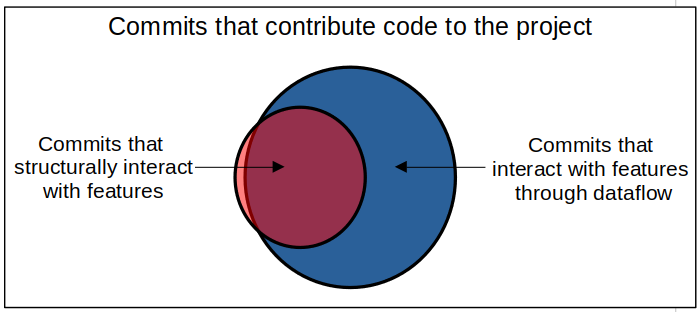
\includegraphics[height=6cm]{gfx/Commits-of-a-Software-Project.png}
\end{tabular}
\captionof{figure}{Kinds of Commits in a Software Project investigated in this work}
\end{center}

\textsf{In the first two \textbf{RQs} we have discussed different kinds of commits and the ways in which they interact with features. 
Figure 1 showcases them in a venn diagram and illustrates the dependencies and divisions between them.} 

\subsection*{Operationalization}\label{sec:operationalization}

Here, we explain how the proposed RQs from the previous section can be answered.
The general experiment process is the same for all RQs.
At first, we collect data comprimising all structural or dataflow-based commit-feature interactions by creating reports of a specific type for a chosen software project.
The collected data is then processed in order to gain information for each commit or feature in the project, such as the number of interacting commits and size of a feature.
The processed data is used to calculate statistical information, such as the mean and variance, or the strength of a correlation.
To facilitate a faster and better understanding of the processed data and calculated statistics, we display them graphically via distribution or regression plots.
The projects we investigate in this work, for example xz and gzip, are of a small size and are used in a compression domain.
This choice is based on the fact, that our research intends to only lay basic groundwork, where smaller projects can already offer a lot of insight.
Since we only investigate a few projects, we chose them to be of a similar domain, such that a comparison between them makes more sense.
In the following sections, we explain our method of investigation in more detail for each RQ.

\subsubsection*{\textbf{RQ1: How do commits and features structurally interact with eachother?}}

For this RQ, we obviously examine reports comprising structural commit-feature interactions.
From the collected data we extract the size and the number of commits a feature structurally interacts with as well as the number of features a commit structurally interacts with.
Concerning the first property of structural commit-feature interactions mentioned by us, we calculate the mean and variance of the number of commits used to implement a feature.
This gives us an overview of how many commits were used for a feature's development and tells us how much this number varies for different features.
A regression analysis on the relation between the size of a feature and the commits used to implement it, allows us to calculate the strength of their correlation. 
From the commits that structurally interact with features, we calculate the average number of features that a commit interacts with.
Using the calculated average, we can determine if commits are primarily used to change just one feature.
Showing the distribution of the number of features a commit changes, further allows us to see how often commits change just one or more features.
Here, filtering outliers can help produce more sensible data, as commits responsible for refactoring could change many features, while not implementing any functionality. 

\subsubsection*{\textbf{RQ2: How do commits interact with features through dataflow?}}

The projects investigated for dataflow-based commit-feature interactions are the same projects as investigated for structural commit-feature interactions.
This choice gives us more insight into a single project and allows us to combine both analysis results as will be discussed below.
For this RQ, we consider all commits that currently contribute code to the repository, 
which we can extract from high level repository information of the project.
We process the collected data, such that, for each commit, we save how many features they interact with through dataflow.
Here, we also indicate whether a commit structurally interacts with a feature, which we can simply check by examining the according structural report.
With this information, we are able to separate commits into ones that implement parts of a feature and those that do not. 
We have already dicussed that commits used to implement a feature are much more likely to account for dataflow interactions.
We provide evidence for this by comparing the average amount of features the two types of commits affect through dataflow. 
Besides that we compute what fraction of commits have dataflow-based interactions with other features, once for all commits, once for commits that are part of a feature and once for commits that aren't part of a feature.
This shows how often commits affect features through dataflow based on their intended purpose, e.g. actively changing the functionality of a feature or changing something seemingly unrelated to a feature. 
With the data collected for each commit, we also plot the distribution of how many features they interact with.
This lets us recognize potential outliers, for example commits with much more dataflow interactions than the mean would suggest.

\subsubsection*{\textbf{RQ3: How do authors implement features?}}

Here, we also examine the same projects as in the previous RQs.
That way we can reuse data produced in RQ1 to map each feature to the authors that implemented it.
For RQ1 we have already mapped each feature to the commits it interacts with, e.g. that contribute code to it.
It's possible to extract the authors of these commits by accessing high-level repository information.
This directly gives us the authors that implemented a feature.
With the processed data, we are able to calculate the average number of authors used to implement a feature and plot their distribution for a sound overview.
The size of each feature has also been calculated to answer the previous RQs.
With this information we aim to correlate the size of a feature with the amount of authors that implemented it in a regression analysis.

\iffalse Furthermore we want to estimate the amount of code a developer contributes to a feature.
To accomplish this, we adapt the analysis used to map each feature to the authors that implement them.
When iterating over the commit-feature interactions we not only save the commit, but addtionally save the amount of instructions of that interaction.
When extracting the authors from the commits that were mapped to a feature, we also add up the amount of instructions for each commit.
Now we can estimate the amount of code an author contributes to a feature with the amount of instructions stemming from said code. \fi

\subsection*{Expectations}\label{sec:expectations}

How and to what extent features are used to implement functionality in the to be examined projects is not known and could vary from project to project.
Thus, some results of the dicussed research topics are difficult to predict.
For example, nesting of feature regions inside each other could lead to an increase in the amount of features a commit usually changes.
Due to the discussed best practices of commits, we expect commits to change at most one feature on average if there happens to be little nesting.
Because of the unknown size of features, it's not sensible to give an estimate about the amount of commits needed to implement a feature.
We expect a rather strong positive correlation between the size of a feature and its commits however.
It was mentioned that we examine small projects meaning that the pool of developers is limited in size. 
% Normally, features only encompass a tiny share of a project's overall code. 
Besides that features implement specific functionality that some programmer's might have a better understanding of than others.
This leads us to the expectation that a feature is implemented by a small share of all developers contributing to a project.
Because of the small pool of developers and prior research findings, we expect the existence of a main developer that contributes most if not all of the functionality of a feature.
We know that commits structurally interacting with features most likely are part of dataflow interactions with them as well.
Excluding such commits, the extent to which commits interact with features through dataflow depends heavily on what fraction of the code space is made up of feature regions.
The purpose of features is to implement additional and sometimes necessary functionality separate from the main program.
For this they access and change specific data according to their intended functionality.
Provided that feature regions only make up a small portion of the program, we do expect relatively few, albeit important dataflow interactions between commits and features.

\subsection*{Threats to Validity}\label{sec:threats}

There are some potential threats to the internal validity of our gathered data, which stem from our implementation in VaRA. \\
From definition~\ref{def:feature_regions} of feature regions, it follows that we implement feature regions in such a way that any instruction whose execution depends on a configuration variable, is part of a feature region.
However, not every such instruction also implements the functionality of a feature, as can be seen in listing~\ref{lst:feature_region_overapproximation}.
This means that feature regions overapproximate the amount of instructions responsible for a feature's functionality.
Since feature regions are used for computing both structural and dataflow-based commit-feature interactions, they are overapproximated to some extent as well.
Thus, it's possible that commits of structural interactions don't actually implement functionality of a feature and commits of dataflow interactions don't actually affect instructions implementing a feature's functionality through dataflow.
Furthermore \citet{sattler2023seal} explains that our deployed VaRA taint analysis does not necessarily detect all dataflows occuring in a program.
This results in taints being underapproximated, meaning that some instructions are not tainted when they correctly should be.
Thus, some dataflow interactions could be missed by our deployed commit-feature interaction detection. \\
Concerning the external validity of our findings, most dangers come from the selection of which projects we investigate.
Our pool of investigated projects is limited and it's likely that the way commits and features are used in them is different to other projects to some extent.
In previous chapters we have discussed that the chosen projects are rather small and many of them are from the same domain.
This could mean that our findings might not be applicable for projects of larger size or of different domains.
As we already factor in the size of a feature in the analysis of our data, we are able mitigate some doubts about the applicability of our results onto larger projects, as we can scale them accordingly. \\

\begin{lstlisting}[language=python, caption={Feature Region Overapproximation}, label={lst:feature_region_overapproximation}]
1. if FeatureEncryption:                              %\vartriangleright% %FeatureEncryption%
2.    sendEncryptedMessage(message)                   %\vartriangleright% %FeatureEncryption%
3. else:                                              %\vartriangleright% %FeatureEncryption%
4.    sendMessage(message)                            %\vartriangleright% %FeatureEncryption%
\end{lstlisting}

\textsf{The function of \texttt{FeatureEncryption} is to send the message encrypted. According to our definition of feature regions all instructions stemming from the shown lines of code belong to a region of \texttt{FeatureEncryption}, as their execution depends on the configuration variable of \texttt{FeatureEncryption}. However only instructions stemming from the lines 1-2 implement the actual functionality of the feature. Thus our analysis overapproximates the lines 3-4 to also belong to the feature.} 
